\documentclass{article}
\usepackage[T1]{fontenc}
\usepackage{geometry}
\geometry{
	a4paper,
	total={170mm,257mm},
	left=20mm,
	top=20mm,
}
\usepackage{graphicx}
\usepackage{titling}

\title{Summary of Scientific Articles}
\author{Hao ZHANG}
\date{August 29, 2023}

\usepackage{fancyhdr}
\pagestyle{fancy}
\fancypagestyle{plain}{
	\fancyhf{}
	\fancyhead[L]{\thetitle}
	\fancyhead[R]{\theauthor}
	\fancyfoot[L]{\thedate}
	\fancyfoot[C]{\vskip -10pt
\includegraphics[width=1cm]{My_Seal.png}}
	\fancyfoot[R]{\thepage}
}
\fancyhf{}
\fancyhead[L]{\thetitle}
\fancyhead[R]{\theauthor}
\fancyfoot[L]{\thedate}
\fancyfoot[C]{\vskip -10pt
\includegraphics[width=1cm]{My_Seal.png}}
\fancyfoot[R]{\thepage}
\makeatletter
\def\@maketitle{
	\newpage
	\null
	\vskip 1em
	\begin{center}
		\let \footnote \thanks
		{\LARGE \@title \par}
		\vskip 1em
	\end{center}
	\par
	\vskip 1em}
\makeatother

\usepackage{lipsum}  
\usepackage{cmbright}

\makeatletter
\renewcommand\paragraph{\@startsection{paragraph}{4}{\z@}%
	{3.25ex \@plus1ex \@minus.2ex}%
	{-1em}%
	{\normalfont\normalsize}}
\makeatother

\begin{document}
	
	\maketitle
	
	\hrule
	\vskip 2em
	\noindent\begin{tabular}{@{}ll}
		Article Title & Building an Ontology of Boardgame Mechanics based on the BoardGameGeek \\ & Database and the MDA Framework\\
		Article Authors & Joshua Kritz, Eduardo Mangeli, Geraldo Xexéo\\
		Publication Information &  SBC – Proceedings of SBGames 2017 | ISSN: 2179-2259
	\end{tabular}
	\vskip 2em
	\noindent\dotfill
	
	\section{The MDA framework and related work}
	
	\subsection{Purpose, function and its three components}
	
	\paragraph*{The MDA (Mechanics, Dynamics, and Aesthetics) framework was created to help designers, researchers, and scholars decompose games into coherent and understandable parts. To this purpose, the framework establishes causal relationships between these classes, in addition to classifying game components.}
	
	\paragraph*{Game elements are classified into three distinct components: mechanics, dynamics, and aesthetics, where the mechanics are the only components that can be directly used by the game designer or developer, and the game mechanics ontology can be seen as a template for constructing the game. In terms of dynamics and aesthetics, game dynamics stem from the player's interaction with the mechanics, while aesthetics stem from the dynamics and are the player's emotional response.}
	
	\subsection{Relationship of the three components}
	
	\paragraph*{The components of the MDA framework and the relationships between them, from the designer's and player's perspectives, are shown in the figure below: }
	
	\begin{figure}[h]
		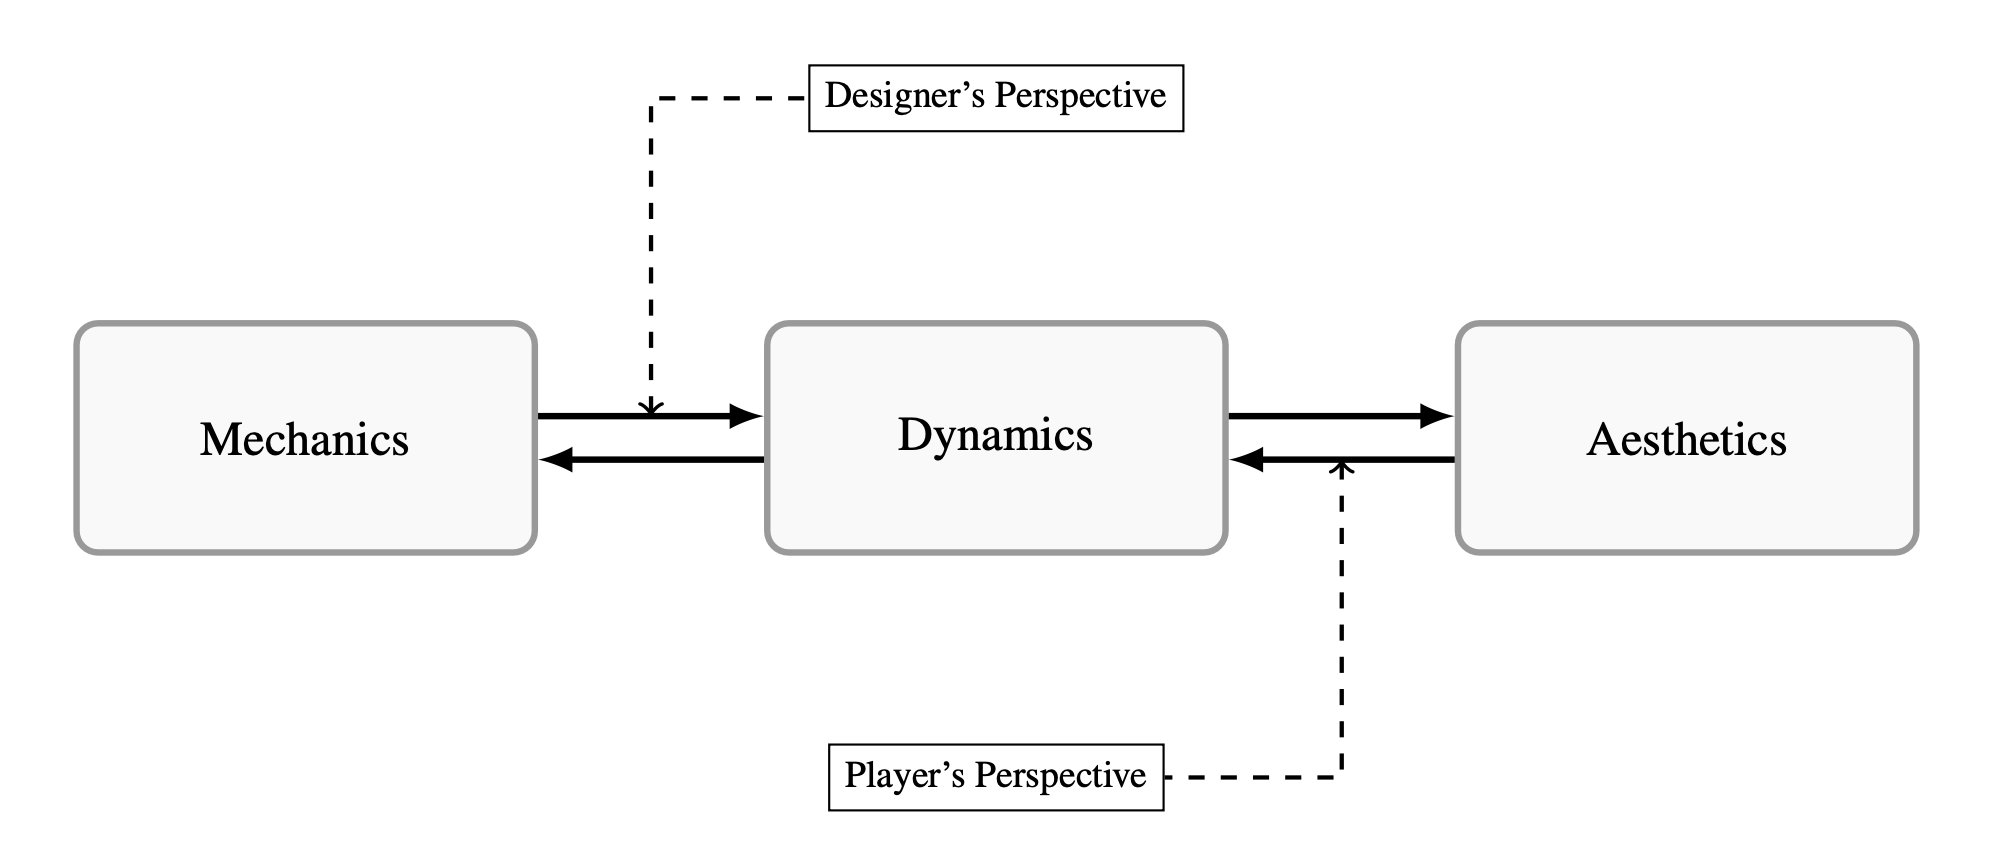
\includegraphics[width=\textwidth]{Figure_1.png}
	\end{figure}
	
	\subsection{Related work}
	
	\paragraph*{There have been attempts to construct game-related ontologies, mainly for video games.}
	
	\paragraph*{The best-known ontology is the Game Ontology Project (GOP), which is "a framework for describing, analyzing, and studying games," and several researchers have constructed role-playing game (RPG) ontologies inspired by the GOP. More recently, the GOP and MDA have also been used to provide an innovative model for digital games, which can also be used in methodologies for board games.}
	
	\section{Board Game Geek Forum}
	
	\paragraph*{Board Game Geek (BGG) is one of the largest and most used board game forums on the Internet, and due to its expansive nature, the BGG database has become a source of information used by scholars and game designers. One of its main functions is to provide a very comprehensive list of board games that have ever appeared, keeping a historical record of the games. On July 22, 2017, the BGG listed 92018 games, over 2536 series, 84 categories, and 51 mechanics.}
	
	\paragraph*{The work in this paper aims to build an ontology of game mechanics based on the mechanical categories introduced in the BGG and the formal concepts in the MDA framework. The main aim of this work is to provide a tool for game designers, academics and others who consider game artifacts as objects of study or are interested in making games.}
	
	\section{Methodology}
	
	\subsection{Principles}
	
	\paragraph*{The methodology used in this paper is based on the MENELAS method, which creates classification trees based on four principles. These principles are similarity, specificity, opposability and unique semantic axis. Among them, the first three principles are used to categorize some BGG mechanics into superclasses and decompose them into subclasses so as to naturally create a tree structure with a unique root, and the normalization of BGG mechanics will contribute to this structuring, which will play an important role in the understanding of the natural and pure-theoretical relations that determine the ontology.}
	
	\subsection{Limitations of the rules}
	
	\paragraph*{There are some rules to limit the scope of the ontology, e.g., only concepts recognizable in BGG should appear as leaves of the ontology; higher-level concepts should be based on the MDA framework or other references; composite mechanics should be decomposed into its different constituents, etc.}
	
	\section{Ontology construction}
	
	\subsection{Top concepts}
	
	\paragraph*{Detailing the ontology in this paper, the first layer of the architecture consists of two very general mechanisms taken directly from the MDA framework: algorithms and data representations. The former is the general mechanism of the game process, categorized into actions, goals and rulesets; the latter is the general mechanism of storing and transferring information in the game, categorized into components and resources. They will be further divided according to the explanation of the former in the framework and the references.}
	
	\subsection{Partial relationships}
	
	\paragraph*{During the creation of the ontology, many partial relationships can be easily identified, as some of the classes actually come from BGG mechanics, which derive from related classes that only appear in the description and therefore need to be defined as mechanics. In this way, they form a natural relationship with each other. Of course, other partial relationships require more effort to analyze whether they actually occur in a particular instance.}
	
	\subsection{Some minor shortcomings}
	
	\paragraph*{Some BGG game mechanisms do not appear in the list of concepts or definitions in the Game Mechanisms Ontology. Due to the limitations of the list of BGG mechanics, the ontology omits some mechanics.}
	
	\section{Future direction}
	
	\paragraph*{The proposed ontology is an ongoing effort that must be refined over time, as it is intended to cover a wide range of ever-innovating games. In order to refine the ontology, the researchers will look for other sources of mechanisms to extend the ontology, aiming to improve the existing ontology by creating more relationships and enhancing existing ones.}
	
\end{document}
